\section{处理机的调度与死锁}

\begin{frame}[fragile]{CH3 处理机的调度与死锁}
  \begin{easylist} \easyitem
    & 3.1 处理机调度的基本概念
    & 3.2 调度算法
    & 3.3 实时调度
    & 3.4 多处理机系统中的调度
    & 3.5 产生死锁的原因和必要条件
    & 3.6 预防死锁的办法
    & 3.7 死锁的检测与解除
  \end{easylist}
\end{frame}


\subsection{3.1 处理机调度的基本概念}
\begin{frame}[fragile]{3.1 处理机调度的基本概念}
  \begin{easylist} 
    & 进程调度的定义和目标
    & 高级、中级和低级调度
    & 调度队列模型
    & 选择调度方式和调度算法的若干准则
  \end{easylist}
\end{frame}

\begin{frame}[fragile]{进程调度的定义}
  \begin{easylist} \easyitem
    & 单CPU环境下,任一时刻只能有一个进程处于执行状态,如何确定在某一时刻由哪个
    进程执行?
    & 调度:
    && 根据特定目标选择下一个要运行的进程
    && 调度的级别或者说粒度问题?
  \end{easylist}
\end{frame}

\begin{frame}[fragile]{高级、中级和低级调度}
  \begin{easylist} \easyitem
    & 高级调度
    && 作业调度、长程调度、接纳调度
    & 中级调度
    & 低级调度
    && 进程调度,短程调度
    \vspace{1cm}
    & 运行频率:低 $\backsim$ 中 $\backsim$ 高
  \end{easylist}
\end{frame}


\begin{frame}[fragile]{高级调度}
  \begin{easylist} \easyitem
    & 确定将哪些外存作业调入内存之中,进而创建PCB等,插入就绪队列
    & 一般用于批处理系统,分/实时系统一般直接入内存,无此环节
    \vspace{1cm}
    & 调度特性
    && 1.接纳作业数(内存驻留数)
    &&& 太多 $\Rightarrow$  周转时间T长
    &&& 太少 $\Rightarrow$  系统效率低
    && 2.接纳策略:
    &&& 即采用何种调度算法:FCFS、短作业优先、基于作业优先权的调度、响应比高者优先等
  \end{easylist}
\end{frame}


\begin{frame}[fragile]{低级调度}
  \begin{easylist}
    & 主要是由分派程序(Dispatcher)分派处理机。
    & 1.非抢占方式:
    && 简单,实时性差  (如win31)
    & 2.抢占方式
    && (1)时间片原则
    && (2)优先权原则
    && (3)短作业优先原则。   
  \end{easylist}
\end{frame}


\begin{frame}[fragile]{中级调度}
  \begin{easylist} \easyitem
    & 为提高系统吞吐量和内存利用率而引入的内外存对换功能(换出时,进程为挂起或就绪驻外状态) 
    & 典型代表:存储器管理中的对换功能
  \end{easylist}
\end{frame}


\begin{frame}[fragile, allowframebreaks]{选择调度方式和算法的准则}
  \begin{easylist} \easyitem
    & 一、面向用户的准则: 周转时间、响应时间
    && 1.周转时间短(常用于批处理系统)
    &&& 概念:作业从提交到完成的时间,分为:
    &&&& (1)驻外等待调度时间
    &&&& (2)驻内等待调度时间
    &&&& (3)执行时间
    &&&& (4)阻塞时间
    && 2.响应时间快:(对交互型作业)
    &&& 概念:键盘提交请求到首次响应时间
    &&&& (1)输入传送时间
    &&&& (2)处理时间
    &&&& (3)响应传送时间
    && 3.截止时间的保证(特别于实时系统)
    && 4.优先权准则:(即需要抢占调度)

    & 二、面向系统的准则
    && 1.吞吐量高(特别于批处理):单位时间完成作业数
    && 2.处理机利用率好:(因CPU贵,特别对于大中型多用户系统)
    && 3.各类资源的平衡利用。(?折算标准)    
  \end{easylist}

  \vspace{1cm}

  早期更看重处理机利用率(面向系统优先),后来更注重用户体验。
\end{frame}


\subsection{3.2 调度算法}
\begin{frame}[fragile]{3.2 调度算法}
  \begin{easylist} \easyitem
    & 3.2.1 先来先服务和短作业优先调度算法
    & 3.2.2 高优先权优先调度算法
    & 3.2.3 基于时间片的轮转调度算法
    \vspace{1cm}
    & \em{OS中调度的实质是一种资源分配}    
  \end{easylist}
\end{frame}

\begin{frame}[fragile]
  \frametitle{Scheduler and Dispatcher}
  \begin{easylist}
    & In simple term, Scheduler will select the process from ready queue and
    dispatcher will do the labor work of saving and loading of new process into
    the cpu.

    From: \url{https://www.quora.com/OS-What-is-the-difference-between-a-scheduler-and-a-dispatcher}
  \end{easylist}
\end{frame}


\begin{frame}[fragile]{3.2.1 先来先服务和短作业优先}
  \begin{easylist} \easyitem
   & 1.FCFS
   && 特点:简单,有利于长作业 即CPU繁忙型作业
   & 2.短作业/进程优先调度算法:SJ(P)F
   && 提高了平均周转时间和平均带权周转时间(从而提高了系统吞吐量)
   && 特点:对长作业不利,有可能得不到服务(饥饿)
   && 估计时间不易确定 
  \end{easylist}
\end{frame}


\begin{frame}[fragile]{FCFS示例}
  \begin{tabular}{|c|p{28pt}|p{28pt}|p{36pt}|p{28pt}|p{28pt}|p{36pt}|}
    \hline \rowcolor{yellow!30}
    进程名 & 到达时间 & 服务时间 & 开始执行时间 & 完成时间 & 周转时间 & 带权周转时间 \\ \hline
    A & 0 & 1 &  &  &  &  \\ \hline
    B & 1 & 100 &  &  &  & \\ \hline
    C & 2 & 1 &  &  &  & \\ \hline
    D & 3 & 100 &  &  &  & \\ \hline
  \end{tabular}
\end{frame}

\begin{frame}[fragile]{FCFS示例}
  \begin{tabular}{|c|p{28pt}|p{28pt}|p{36pt}|p{28pt}|p{28pt}|p{36pt}|}  
    \hline \rowcolor{yellow!30}
    进程名 & 到达时间 & 服务时间 & 开始执行时间 & 完成时间 & 周转时间 & 带权周转时间 \\ \hline
    A & 0 & 1 & 0 & 1 & 1 & 1 \\ \hline
    B & 1 & 100 & 1 & 101 & 100 & 1\\ \hline
    C & 2 & 1 & 101 & 102 & 100 & 100\\ \hline
    D & 3 & 100 & 102 & 202 & 199 & 1.99\\ \hline
  \end{tabular}
\end{frame}


\begin{frame}[fragile]{FCFS和SJF的比较}
  \begin{tabular}{|c|l|p{0.8cm}|p{0.8cm}|p{0.8cm}|p{0.8cm}|p{0.8cm}|c|}
    \hline
    \multirow{3}{*}{} & 进程名 & A & B & C & D & E & 平均 \\ \cline{2-8}
    & 到达时间 & 0 & 1 & 2 & 3 & 4 & \\ \cline{2-7}
    & 服务时间 & 4 & 3 & 5 & 2 & 4 & \\ \hline \hline

    \multirow{3}{*}{FCFS} & 完成时间 & ~ &  &  &  &  &  \\ \cline{2-8}
    & 周转时间 &  &  &  &  &  &  \\ \cline{2-8}
    & 带权周转时间 &  &  &  &  &  &  \\ \hline \hline

    \multirow{3}{*}{SJF} & 完成时间 &  &  &  &  &  &  \\ \cline{2-8}
    & 周转时间 &  &  &  &  &   &  \\ \cline{2-8}
    & 带权周转时间 &  &  &  &  &  &  \\ \hline
  \end{tabular}
\end{frame}


\begin{frame}[fragile]{FCFS和SJF的比较}
  \begin{tabular}{|c|l|p{0.8cm}|p{0.8cm}|p{0.8cm}|p{0.8cm}|p{0.8cm}|c|}
    \hline
    \multirow{3}{*}{} & 进程名 & A & B & C & D & E & 平均 \\ \cline{2-8}
    & 到达时间 & 0 & 1 & 2 & 3 & 4 & \\ \cline{2-7}
    & 服务时间 & 4 & 3 & 5 & 2 & 4 & \\ \hline \hline

    \multirow{3}{*}{FCFS} & 完成时间 & 4 & 7 & 12 & 14 & 18 &  \\ \cline{2-8}
    & 周转时间 & 4 & 6 & 10 & 11 & 14 & 9 \\ \cline{2-8}
    & 带权周转时间 & 1 & 2 & 2 & 5.5 & 3.5 & 2.8 \\ \hline \hline

    \multirow{3}{*}{SJF} & 完成时间 & 4 & 9 & 18 & 6 & 13 &  \\ \cline{2-8}
    & 周转时间 & 4 & 8 & 16 & 3 &  9 & 8 \\ \cline{2-8}
    & 带权周转时间 & 1 & 2.67 & 3.2 & 1.5 & 2.25 & 2.1 \\ \hline
  \end{tabular}
\end{frame}



\begin{frame}[fragile]{3.2.2高优先权优先调度算法}
  \begin{easylist}
    & 优先权调度算法类型
    && 非抢占式优先权算法
    && 抢占式优先权算法,实时性更好。
    & 优先权类型
    && 静态优先权
    && 动态优先权
    & 高响应比优先
  \end{easylist}
\end{frame}

\begin{frame}[fragile, allowframebreaks]{优先权类型}
  \begin{easylist} \easyitem
    & 1.静态优先权:
    && 进程优先权在整个运行期不变。
    && 确定优先权依据
    &&& (1)进程类型
    &&& (2)进程对资源的需求;
    &&& (3)根据用户需求。
    && 特点:简单,但低优先权作业可能长期不被调度。

    \newpage
    & 2.动态优先权:
    && 如: 优先权随执行时间而下降,随等待时间而升高。
    && 响应比$R_p$=(等待时间+服务时间)/服务时间  作为优先权
    && 优点:长短兼顾    
    &&  缺点:需计算$R_p$   
  \end{easylist}
\end{frame}

\begin{frame}[fragile, allowframebreaks]{高响应比优先算法}
  \begin{easylist} \easyitem
    & 特点
    && 响应比$R_p =(tw+ts)/ts$
    && (1) 短作业$R_P$大。
    && (2) ts(要求服务时间)相同的进程间相当于FCFS。
    && (3) 长作业等待一段时间仍能得到服务。
  \end{easylist}
\end{frame}


\begin{frame}[fragile, allowframebreaks]{3.2.3 基于时间片的轮转调度算法}
  \begin{easylist} \easyitem
    & 1.时间片轮转
    && 时间片大小的确定
    &&& 太大:退化为FCFS;
    &&& 太小:系统开销过大
    && 系统对响应时间的要求;
    && 就绪队列中进程的数目;
    && 系统的处理能力:(应保证一个时间片处理完常用命令)
    \newpage
    & 2.多级反馈队列调度
    && 特点:长、短作业兼顾,有较好的响应时间
    &&& (1)短作业一次完成;
    &&& (2)中型作业周转时间不长;
    &&& (3)大型作业不会长期不处理。
  \end{easylist}
\end{frame}


\begin{frame}[fragile]{多级队列反馈调度算法}
  \begin{center}
  \begin{tikzpicture}[c/.style={draw,thick, minimum width=3cm, minimum height=0.75cm}]
    \draw[] node[c] (q1) {就绪队列1}
    node[c, below=1 of q1] (q2) {就绪队列2}
    node[c, below=1 of q2] (q3) {就绪队列3}
    node[c, below=1 of q3] (qn) {就绪队列n};

    \draw[-Latex] (q1.west) ++(-1,0) --(q1);
    \path[-Latex] (q1.east) ++(0,0.1) edge node[above]{$S_1$} ++(2.5,0) node[right=2.5cm]{至CPU};
    \draw[-latex] (q1.east) ++(0,-0.1) -- ++(1,0) -- ++(0,-0.8)  --++(-5,0) |- (q2.west);

    \path[-Latex] (q2.east) ++(0,0.1) edge node[above]{$S_2$} ++(2.5,0) node[right=2.5cm]{至CPU};
    \draw[-latex] (q2.east) ++(0,-0.1) -- ++(1,0) -- ++(0,-0.8)  --++(-5,0) |- (q3.west);

    \path[-Latex] (q3.east) ++(0,0.1) edge node[above]{$S_3$} ++(2.5,0) node[right=2.5cm]{至CPU};
    \draw[-latex, dotted, thick] (q3.east) ++(0,-0.1) -- ++(1,0) -- ++(0,-0.8)  --++(-5,0) |- (qn.west);

    \path[-Latex] (qn.east) ++(0,0.1) edge node[above]{$S_n$} ++(2.5,0) node[right=2.5cm]{至CPU};
    \draw[-latex] (qn.east) ++(0,-0.1) -- ++(1,0) -- ++(0,-0.8) --++(-5,0) |- (qn.190);

    \node[below=0.6 of qn]{时间片:$S_1 < S_2 <S_3$};
  \end{tikzpicture}
  \end{center}
\end{frame}


\begin{frame}[fragile]{3.3 实时调度}
  \begin{easylist}
    & 前面提到的调度算法,不能满足实时系统的要求
  \end{easylist}
\end{frame}

\begin{frame}[fragile, allowframebreaks]{3.3.1 实现实时调度的基本条件}
  \begin{easylist}
    & 1.提供必要的调度信息
    && (1) 就绪时间;
    && (2) 开始/完成截止时间;
    && (3) 处理时间;
    && (4) 资源要求;
    && (5) 优先级;
    & 2.系统处理能力强
    $$\sum_{i=1}^{m} \dfrac{C_i}{P_i} \leqslant 1 (\text{单处理器})~~or~~ \sum_{i=1}^{m} \dfrac{C_i}{P_i} \leqslant N (\text{多处理器})$$
    && $C_i$为处理时间,$P_i$为周期时间(基于周期性实时任务)
    
    \newpage
    & 3.采用抢占调度方式
    && 剥夺方式:一般都采用此
    && 非剥夺方式(实现简单):一般应使实时任务较小,以及时放弃CPU。
    & 4.具有快速切换机制
    && 具有快速响应外部中断能力
    && 快速任务分派
  \end{easylist}
\end{frame}

\begin{frame}[fragile]{3.3.2 实时调度算法的分类}
  \begin{easylist} \easyitem
    & 1. 非抢占式调度算法
    && 时间片轮转   			秒级
    && 非抢占优先权(协同)  	秒~毫秒级
    & 2. 抢占式调度算法
    && 时钟中断抢占优先权 		毫秒级
    &&& 基于抢占点抢占
    && 立即抢占immediate preemption   毫秒~微秒级
    &&& 只要不在临界区即抢占(中断引发)
  \end{easylist}
\end{frame}


\begin{frame}[fragile]{调度时机图例}
  \begin{center}
    \scalebox{0.85}{
      \begin{tikzpicture}[c/.style={draw,thick, minimum width=2cm, minimum height=0.75cm}]
        \draw[] node[c, fill=yellow!20] (p1) {进程1}
        node[c, right=0 of p1] (p2) {进程2}
        node[minimum width=1.5cm, right=0 of p2] (pi) {$\cdots$}
        node[c, right=0 of pi] (pn) {进程$n$}
        node[c, right=0 of pn, fill=red!20] (pnow) {实时进程};

        \draw[-Latex, dotted, very thick] (p1.north) ++(0,0.6) node[above](req) {实时进程要求调度} -- (p1); 
        \draw[-Latex, dotted, very thick] (pn.east) ++(0,0.975) node[above](schedule) {调度实时进程运行} -- ++(0,-0.6); 
        \draw[] (p1.south) -- ++(0,-1) ++(0,0.2) coordinate(a);
        \draw[] (pn.east) ++(0,-0.375) -- ++(0,-1)  ++(0,0.2) coordinate(b);
        \path[<->] (a) edge node[above] {调度时间} (b);
        \node[below=1.2cm of pi] {(a) 非抢占轮转调度};
      \end{tikzpicture}
    }
    \vspace{0.5cm}

    \pause
    \scalebox{0.85}{
      \begin{tikzpicture}[c/.style={draw,thick, minimum width=3cm, minimum height=0.75cm}]
        \draw[] node[c, minimum width=4cm, fill=yellow!20] (p1) {当前进程}
        node[c, right=0 of p1] (pnow) {实时进程};

        \draw[-Latex, dotted, very thick] (p1.north) ++(-1,0.6) node[above](req) {实时进程要求调度} -- ++(0,-0.6); 
        \draw[-Latex, dotted, very thick] (p1.east) ++(0,0.975) node[above, xshift=1cm](schedule) {当前进程运行完成} -- ++(0,-0.6); 
        \draw[] (p1.south) ++(-1,0) -- ++(0,-1) ++(0,0.2) coordinate(a);
        \draw[] (p1.east) ++(0,-0.375) -- ++(0,-1)  ++(0,0.2) coordinate(b);
        \path[<->] (a) edge node[above] {调度时间} (b);
        \node[below=1.2cm of p1, xshift=1.5cm] {(b) 非抢占优先权调度};
      \end{tikzpicture}
    }
  \end{center}
\end{frame}


\begin{frame}[fragile]{调度时机图例}
  \begin{center}
    \scalebox{0.85}{
      \begin{tikzpicture}[c/.style={draw,thick, minimum width=3cm, minimum height=0.75cm}]
        \draw[] node[c, minimum width=4cm, fill=yellow!20] (p1) {当前进程}
        node[c, right=0 of p1] (pnow) {实时进程};

        \draw[-Latex, dotted, very thick] (p1.north) ++(-1,0.6) node[above](req) {实时进程要求调度} -- ++(0,-0.6); 
        \draw[-Latex, dotted, very thick] (p1.east) ++(0,0.975) node[above, xshift=1cm](schedule) {时钟中断到达时} -- ++(0,-0.6); 
        \draw[] (p1.south) ++(-1,0) -- ++(0,-1) ++(0,0.2) coordinate(a);
        \draw[] (p1.east) ++(0,-0.375) -- ++(0,-1)  ++(0,0.2) coordinate(b);
        \path[<->] (a) edge node[above] {调度时间} (b);
        \node[below=1.2cm of p1, xshift=1.5cm] {(c) 基于时钟中断抢占的优先权抢占调度};
      \end{tikzpicture}
    }
    \vspace{0.5cm}

    \pause
    \scalebox{0.85}{
      \begin{tikzpicture}[c/.style={draw,thick, minimum width=3cm, minimum height=0.75cm}]
        \draw[] node[c, minimum width=4cm, fill=yellow!20] (p1) {当前进程}
        node[c, right=0 of p1] (pnow) {实时进程};

        \draw[-Latex, dotted, very thick] (p1.north) ++(-1,0.6) node[above](req) {实时进程要求调度} -- ++(0,-0.6); 
        \draw[-Latex, dotted, very thick] (p1.east) ++(0,0.975) node[above, xshift=1cm](schedule) {抢占时刻(其它中断)} -- ++(0,-0.6); 
        \draw[] (p1.south) ++(-1,0) -- ++(0,-1) ++(0,0.2) coordinate(a);
        \draw[] (p1.east) ++(0,-0.375) -- ++(0,-1)  ++(0,0.2) coordinate(b);
        \path[<->] (a) edge node[above] {调度时间} (b);
        \node[below=1.2cm of p1, xshift=1.5cm] {(d) 立即抢占优先权调度};
      \end{tikzpicture}
    }
  \end{center}
\end{frame}


\begin{frame}[fragile]{3.3.3 常用的几种实时调度算法}
  \begin{easylist} \easyitem
    & 1. 最早截止时间优先EDF (earliest deadline first)算法
    && 根据任务的截止时间来确定任务的优先级
    && 截止时间越早,优先级越高
    && 可以是抢占式或非抢占式
  \end{easylist}
\end{frame}

\begin{frame}[fragile]{最早截止时间优先EDF例}
  \begin{center}
    \begin{tikzpicture}[c/.style={draw,thick, fill=red!5, minimum width=2cm, minimum height=0.75cm}]
      \coordinate (n) at (0,0);
      \draw[left=1.5 of n] node (label1){任务执行} node[c,right=1 of n] (n1) {1} node[c, right=0 of n1] (n3) {3} node[c, right=0 of n3] (n4) {4} node[c, right=0 of n4] (n2) {2};
      \draw[very thick, -Latex] (n1.south) ++(-2,0)--++(10,0) node[right]{$t$};
      \draw[] node[above=0.5 of label1, xshift=0.35cm]{开始截止时间} node[below=of label1]{任务到达};
      \draw[thick,->] (n1.north) -- ++(0,1) node[above] {1};
      \draw[thick,->] (n3.north) -- ++(0,1) node[above] {3};
      \draw[thick,->] (n4.north) -- ++(0,1) node[above] {4};
      \draw[thick,->] (n2.north) -- ++(0,1) node[above] {2};

      \draw[thick,<-, blue] (n.south) ++(1,-0.5)-- ++(0,-1) node[below] {1};
      \draw[thick,<-, blue] (n.south) ++(1.8,-0.5)-- ++(0,-1) node[below] {2};
      \draw[thick,<-, blue] (n.south) ++(2.5,-0.5)-- ++(0,-1) node[below] {3};
      \draw[thick,<-, blue] (n.south) ++(4.5,-0.5) -- ++(0,-1) node[below] {4};
    \end{tikzpicture}

    EDF算法用于非抢占调度方式
  \end{center}
\end{frame}


\begin{frame}[fragile]{2 最低松弛度优先LLF算法}
  \begin{easylist} \easyitem
    & 松弛度:
    && 若A进程需在200ms时完成,其本身运行需要100ms,当前时刻是10ms,则A的松弛度为:200-100-10=90
    && 主要用于可抢占的调度方式中
    & 例:两个周期性实时任务A、B,A要求每20ms执行一次,每次需要10ms,B要求每
    50ms执行一次,每次需要25毫秒。
    \begin{center}
      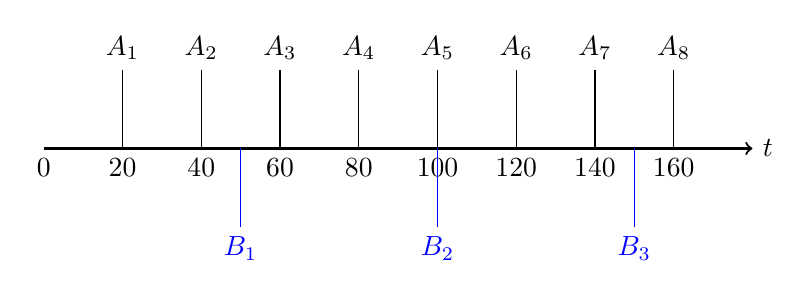
\begin{tikzpicture}[]
        \draw[->, thick] (0,0)--(9,0) node[right] {$t$};
	\draw node[below] at (0,0) {0};

	\draw node[below] at (1,0) {20} (1,0)--++(0,1) node[above]{$A_1$};
        \draw node[below] at (2,0) {40} (2,0)--++(0,1) node[above]{$A_2$};
        \draw node[below] at (3,0) {60} (3,0)--++(0,1) node[above]{$A_3$};
        \draw node[below] at (4,0) {80} (4,0)--++(0,1) node[above]{$A_4$};
        \draw node[below] at (5,0) {100} (5,0)--++(0,1) node[above]{$A_5$};
        \draw node[below] at (6,0) {120} (6,0)--++(0,1) node[above]{$A_6$};
        \draw node[below] at (7,0) {140} (7,0)--++(0,1) node[above]{$A_7$};
        \draw node[below] at (8,0) {160} (8,0)--++(0,1) node[above]{$A_8$};

        \draw[blue] (2.5,0)--++(0,-1) node[below]{$B_1$};
        \draw[blue] (5,0)--++(0,-1) node[below]{$B_2$};
        \draw[blue] (7.5,0)--++(0,-1) node[below]{$B_3$};
      \end{tikzpicture}

      A/B任务每次必须完成的时间
    \end{center}
  \end{easylist}
\end{frame}


\begin{frame}[fragile]{最低松弛度优先LLF算法(2)}
  \begin{center}
    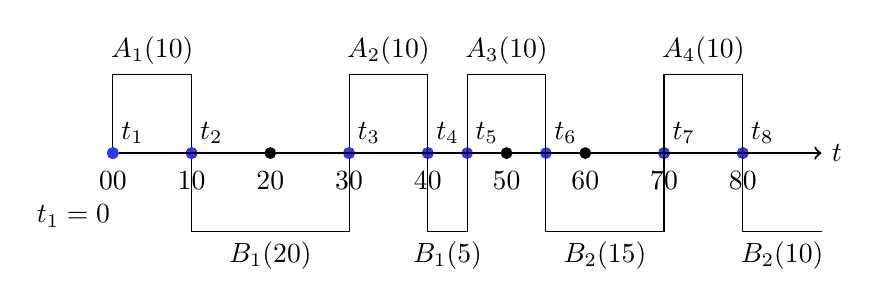
\begin{tikzpicture}[c/.style={draw,thick, fill=black, minimum width=0.12cm,inner sep=0, shape=circle}]
      \foreach \x in {0,1,...,8} 
      \draw[] node[c] at(\x,0) {} node[yshift=-0.35cm] at (\x,0){${\x0}$};

      \foreach \x/\y in {0/1, 1/2, 3/3, 4/4, 4.5/5, 5.5/6, 7/7,8/8}
      \draw[] node[c,blue!80] (t\y) at (\x,0){} node[xshift=0.25cm,yshift=0.25cm] at (t\y){$t_\y$};

      \draw[->, thick] (t1)--(9,0) node[right] {$t$};

      \draw[] (t1)--++(0,1)--++(1,0) --(t2)--++(0,-1)--++(2,0)--(t3)--++(0,1)--++(1,0)--++(0,-2)--++(0.5,0)--++(0,2)--++(1,0)--++(0,-2)--++(1.5,0)--++(0,2)--++(1,0)--++(0,-2)--++(1,0);

      \draw node[] at(-0.5,-0.8) {$t_1 = 0$};
      \draw node[above=1cm] at(0.5,0) {$A_1(10)$};
      \draw node[below=1cm] at(2,0) {$B_1(20)$};
      \draw node[above=1cm] at(3.5,0) {$A_2(10)$};
      \draw node[below=1cm] at(4.25,0) {$B_1(5)$};

      \draw node[above=1cm] at(5,0) {$A_3(10)$};
      \draw node[below=1cm] at(6.25,0) {$B_2(15)$};
      \draw node[above=1cm] at(7.5,0) {$A_4(10)$};
      \draw node[below=1cm] at(8.5,0) {$B_2(10)$};
    \end{tikzpicture}
  \end{center}
\end{frame}

\subsection{3.4 多处理机系统中的调度}
\begin{frame}[fragile]{3.4 多处理机系统中的调度}
  \begin{easylist} \easyitem
    & 提供计算机系统性能的主要途径
    && 提高元器件运行速度
    && 改进计算机体系结构
    \vspace{1cm}
    && 20世纪70年代出现多处理器系统MPS
    &&& Multi-Processor Systems
  \end{easylist}
\end{frame}


\begin{frame}[fragile]{3.4.1 多处理器系统的类型}
  MPS: MultiProcessor System
  \begin{easylist} \easyitem
    & 1.紧密耦合MPS和松弛耦合MPS
    && 紧密耦合
    &&& 共享RAM和I/O
    &&& 高速总线和交叉开关连接
    && 松弛耦合
    &&& 独立RAM和I/O
    &&& 通道和通信线路连接
    & 2.对称MPS和非对称MPS
    && 对称多处理器系统(SMPS: Symmetric MultiProcessor System)
    && 非对称多处理器系统
  \end{easylist}
\end{frame}

\begin{frame}[fragile]{3.4.2 进程分配方式}
  \begin{easylist} \easyitem
    & 1.对称多处理器系统(SMPS)中进程分配方式
    && 静态分配
    && 动态分配
    &&& 可防止系统中多个处理器忙闲不均
    & 2.非SMPS中进程分配方式
    && 多采用主从方式(Master -- Slave)
    && 进程调度在主处理器上执行
    && 有潜在的不可靠性
  \end{easylist}
\end{frame}


\begin{frame}[fragile]{3.4.3 进程(线程)调度方式}
  \begin{enumerate}
  \item 自调度(Self-Scheduling)
  \item 成组调度方式(Gang Scheduling)
  \item 专用处理器分配方式
  \end{enumerate}
\end{frame}


\begin{frame}[fragile]{1.自调度(Self-Scheduling)}
  \begin{easylist} \easyitem
    & 各个处理机自行在就绪队列中取任务。
    & 特点;简单,分布式调度,调度算法可采用前述方法,多个CPU利用率都不错(不会闲)
    & 但:
    && 瓶颈问题,(单队列)
    && 低效性;(需拷贝现场)
    && 线程切换频繁(当线程合作时,各线程并行的条件不容易满足) 
  \end{easylist}
\end{frame}


\begin{frame}[fragile]{2 成组调度方式(Gang Scheduling)}
  \begin{easylist} \easyitem
    & 将一个进程中的一组线程,每次分派时同时分派到一组处理机上执行,在剥夺处理机
    时也同时对这一组线程执行
    & 优点:
    && (1) 对相互合作的进(线)程组调度,可以减小切换,减小系统开销。
    && (2) 每次分配一组CPU,减少了调度频率。
    & 成组调度如何为应用程序分配时间?
    && (1) 面向程序
    && (2) 面向线程:使处理机利用率更高。 
  \end{easylist}
\end{frame}


\begin{frame}[fragile]{2 成组调度方式(Gang Scheduling)}
  \begin{center}
 \begin{columns}[onlytextwidth,T]
    \begin{column}{0.45\textwidth}
      \begin{tabular}{|c|c|c|}
        \hline
        ~ & 程序A & 程序B \\ \hline
        $CPU_1$ & 线程1 & 线程2 \\ \hline
        $CPU_2$ & 线程2 & 空闲 \\ \hline
        $CPU_3$ & 线程3 & 空闲 \\ \hline
        $CPU_4$ & 线程4 & 空闲 \\ \hline
        时间 & 1/2 & 1/2 \\ \hline
      \end{tabular}

      \hspace{1cm}浪费$\dfrac{3}{8} = 37.5\%$
    \end{column}
    \begin{column}{0.45\textwidth}
 \begin{tabular}{|c|c|c|}
        \hline
        ~ & 程序A & 程序B \\ \hline
        $CPU_1$ & 线程1 & 线程2 \\ \hline
        $CPU_2$ & 线程2 & 空闲 \\ \hline
        $CPU_3$ & 线程3 & 空闲 \\ \hline
        $CPU_4$ & 线程4 & 空闲 \\ \hline
        时间 & 4/5 & 1/5 \\ \hline
      \end{tabular}
      
      \hspace{1cm}浪费$\dfrac{1}{5} \times \dfrac{3}{4} = 15\%$
    \end{column}
  \end{columns}
  \end{center}

  \begin{easylist}
    & 面向应用程序:每个程序各获得$50\%$执行时间
    & 面向线程:两个程序共有5个线程,第一个程序获得$4/5$,第二个获得$1/5$
  \end{easylist}

\end{frame}

\begin{frame}[fragile]{3 专用处理器分配方式}
  \begin{easylist} \easyitem
    & 为进程中的每个线程都固定分配一个CPU,直到该线程执行完毕
    & 引入:
    && 多处理机系统,每个处理机已不再属宝贵资源。
    & 特点:
    && 每个进(线)程专用处理机,使其切换小,提高效率。
    & 主要用于大型计算,实时系统
  \end{easylist}
\end{frame}

\begin{frame}[fragile]{Next}
~  
\end{frame}


\subsection{3.5 产生死锁的原因和必要条件}
\begin{frame}[fragile]{3.5 产生死锁的原因和必要条件}
  \begin{easylist} \easyitem
    & 并发可以改善系统的资源利用率,但可能发生死锁(Deadlock)
    & 死锁:
    && 多个进程在运行过程中因争夺资源而造成的一种僵局(Deadly-Embrace),当进程处
    于这种僵持状态时,若无外力作用,它们都将无法再向前推进。
  \end{easylist}
\end{frame}


\begin{frame}[fragile]{死锁的产生}
  \begin{easylist} \easyitem
    & Deadlock in the everyday life
  \end{easylist}
  \begin{center}
    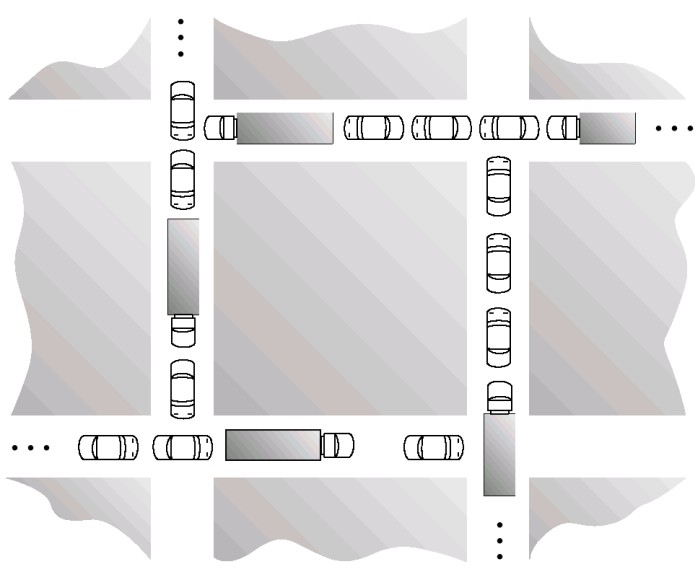
\includegraphics[scale=0.35]{figure/deadlock_car.jpg}
  \end{center}
\end{frame}


\begin{frame}[fragile]{若干死锁的例子}
  \begin{easylist} \easyitem
    & 例1进程推进顺序不当产生死锁
    && 设系统有打印机、读卡机各一台,被进程P和Q共享。两个进程并发执行,按下列
    次序请求和释放资源:
    \begin{center}
      \begin{columns}[T]
        \begin{column}{0.3\textwidth}
          \begin{tabular}{|c|}
            \hline
            进程P \\ \hline
            请求读卡机 \\
            请求打印机\\
            释放读卡机\\
            释放打印机 \\ \hline
          \end{tabular}
        \end{column}
        \begin{column}{0.3\textwidth}
          \begin{tabular}{|c|}
            \hline
            进程Q\\ \hline
            请求打印机\\
            请求读卡机\\
            释放读卡机\\
            释放打印机 \\ \hline
          \end{tabular}
        \end{column}
      \end{columns}
    \end{center}
  \end{easylist}
\end{frame}


\begin{frame}[fragile]{例2 PV操作使用不当产生死锁}
  \begin{center}
    \begin{columns}[T]
      \begin{column}{0.35\textwidth}
        \begin{tabular}{|c|}
          \hline 
          进程P \\ \hline
          $P(S_1)$; \\
          $P(S_2)$; \\
          使用资源$r_1$和$r_2$;\\
          $V(S_1)$; \\
          $V(S_2)$; \\ \hline
        \end{tabular}
      \end{column}
      \begin{column}{0.35\textwidth}
        \begin{tabular}{|c|}
          \hline 
          进程P \\ \hline
          $P(S_2)$; \\
          $P(S_1)$; \\
          使用资源$r_1$和$r_2$;\\
          $V(S_2)$; \\
          $V(S_1)$; \\ \hline
        \end{tabular}
      \end{column}
    \end{columns}
  \end{center}
\end{frame}

\begin{frame}[fragile]{例3 资源分配不当引起死锁}
  \begin{center}
    \begin{tikzpicture}[c/.style={draw,thick, minimum width=1cm, minimum height=0.6cm},
      c2/.style={draw,thick, shape=circle,inner sep=0.1cm, fill=red!20},
      b/.style={draw,thick, fill=black, shape=circle,minimum height=0.15cm, inner sep=0.02cm}]

      \draw[] node[c2] (p1) at(0,0) {$P_1$} 
      node[c2, right=1cm of p1] (p2) {$P_2$} 
      node[c2, right=1cm of p2] (p3) {$P_3$};

      \draw[] node[c] (r1) at(0.7,2) {} node[b] (b1) at(0.7,2) {}  node[above=0.1 of r1]{$R_1$}
      node[c] (r2) at (2.5,2) {} node[b] (b2) at(2.5,2) {}  node[above=0.1 of r2]{$R_2$}
      node[c,minimum height=1cm] (r3) at (0.7, -2) {}  node[b] (b3) at(0.7,-1.8) {}   node[b] (b4) at(0.7,-2.2) {}  node[below=0.1 of r3]{$R_3$}
      node[c,minimum height=1.2cm] (r4) at (2.6, -2.5) {}  node[b] (b5) at(2.6,-2.2) {}   node[b] (b6) at(2.6,-2.5) {}  node[b] (b7) at(2.6,-2.8) {}  node[below=0.1 of r4]{$R_4$};

      \path[-Stealth, thick] (p1) edge (r1) (b1) edge (p2) (p2) edge (r2) (b2) edge (p3)
      (b4) edge (p1) (b3) edge (p2) (p3) edge (r3);
    \end{tikzpicture}
  \end{center}
\end{frame}

\begin{frame}[fragile]{例4 对临时性资源使用不加限制引起死锁}
  \begin{easylist}
    & 进程通信使用的信件是一种临时性资源,如果对信件的发送和接收不加限制,可能引起死锁。
  \end{easylist}
  \begin{center}
    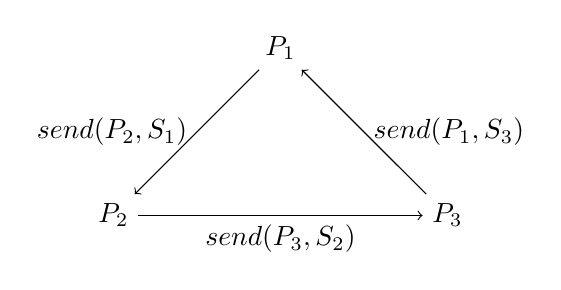
\begin{tikzpicture}[c/.style={draw,thick, minimum width=1cm, minimum height=0.6cm}]
      \draw[] node[] (p1) at(0:0) {$P_1$} node[] (p2) at (225:3) {$P_2$} node[] (p3) at (-45:3) {$P_3$};
      \path[->] (p1) edge node[left]{$send(P_2, S_1)$} (p2)
      (p2) edge node[below]{$send(P_3, S_2)$} (p3)
      (p3) edge node[right]{$send(P_1, S_3)$} (p1);
    \end{tikzpicture}
  \end{center}

   上图中,进程$P_1$需要接收到由$P_3$发送来的资源$S_3$后,就可以向进程$P_2$发送资源$S_1$ $...$
\end{frame}


\begin{frame}[fragile]{3.5.1 产生死锁的原因}
  \begin{enumerate}
  \item 竞争资源引起死锁
  \item 进程推进顺序不当引起死锁
  \end{enumerate}
\end{frame}

\begin{frame}[fragile]{1. 竞争资源引起死锁}
  \begin{easylist} \easyitem
    & 1.可剥夺(CPU、内存,)和非剥夺性(打印机,磁带机)资源
    & 2.竞争非剥夺性资源——可造成死锁 
  \begin{center}
    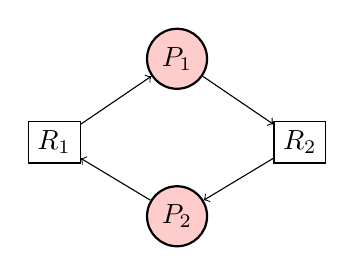
\begin{tikzpicture}[c/.style={draw, thick, fill=red!20, circle, inner sep=0.1cm}]
      \draw[] node[c] (p1) at(0:0) {$P_1$} node[c] (p2) at (-90:2) {$P_2$} node[draw, xshift=-0.5cm] (r1) at (-135:1.5) {$R_1$}  node[draw, xshift=0.5cm] (r2) at (-45:1.5) {$R_2$};
      \path[->] (p1) edge (r2) (r2) edge (p2) (p2) edge (r1) (r1) edge (p1);
    \end{tikzpicture}
  \end{center}
    & 3.竞争临时性资源
    && 永久性资源可重复使用,临时性资源是指由一个进程产生,被另一个进程使用一段
    时间后便无用的资源,也称为消耗性资源。
  \end{easylist}
\end{frame}


\begin{frame}[fragile]{2. 进程推进顺序不当引起死锁}
  \begin{easylist} \easyitem
    & 下图四种颜色的线表示了四种不同的推进顺序,其中红色线所代表的推进顺序会导致死锁
  \end{easylist}
  \begin{center}
    \small
    \begin{tikzpicture}[c/.style={draw,circle, inner sep=0.1cm}]
      \draw[thick] (-0.5, 0)--(9,0) (0,-0.2)--(0,5.5);
      \draw[dotted, thick] node[below] (p11) at (2,0) {$P_1: Req(R_1)$} (2,0)--(2,4.5);
      \draw[dotted, thick] node[below] (p12) at (4,0) {$P_1: Req(R_2)$} (4,0)--(4,4.5);
      \draw[thick] node[below] (p13) at (6,0) {$P_1: Rel(R_1)$} (6,0)--(6,0.75);
      \draw[thick] node[below] (p14) at (8,0) {$P_1: Rel(R_2)$} (8,0)--(8,0.75);

      \draw[dotted, thick] node[left] (p21) at (0,2) {$P_2: Req(R_2)$} (0,2)--(5.5,2);
      \draw[dotted, thick] node[left] (p22) at (0,3) {$P_2: Req(R_1)$} (0,3)--(8.5,3);
      \draw[thick] node[left] (p23) at (0,4) {$P_2: Rel(R_2)$} (0,4)--(0.2,4);
      \draw[thick] node[left] (p24) at (0,5) {$P_2: Rel(R_1)$} (0,5)--(0.2,5);

      \draw[line width=1.2pt, blue,->] (0.2, 0.5)--(8.5,0.5)--(8.5,5.5);
      \draw[line width=1.2pt, purple!90,->] (0.5, 0.2)--(0.5,5)--(8.7,5);
      \draw[line width=1.2pt,->] (0.75,0.75)--(5.5,0.75)--(5.5,2)--(8,2)--(8,5.2);
      \draw[line width=2pt,->, red] (0.75,0.75)--(0.75,1.5)--(3,1.5)--(3,2.5);
      \draw[->, red] node[shape=ellipse, draw=red, thick] (tip) at(5,4) {进入死锁} (3.1, 2.2)--(tip);
    \end{tikzpicture}
  \end{center}
\end{frame}


\begin{frame}[fragile]{3.5.2 产生死锁的必要条件}
  \begin{easylist} \easyitem
    & 1.互斥条件(Mutual Exclusion)
    && 共享资源不会导致死锁,如只读文件
    && 某些资源,如打印机、磁带等,需要被单个进程互斥访问
    & 2.请求和保持条件(Hold and Wait)
    && 持有等待
    & 3.不剥夺条件(No Preemption)
    && 不能抢占
    & 4.环路等待(Circular Wait)
    && 循环等待
  \end{easylist}
\end{frame}

\begin{frame}[fragile]{3.5.3 处理死锁的基本方法}
  \begin{easylist} \easyitem
    & 不允许死锁发生
    && 1.静态预防;
    &&& 破坏4个条件之一:有效,使资源利用率低。
    && 2.动态避免
    &&& 防止进入不安全态。
    & 允许死锁发生
    && 3. 顺其自然、不予理睬
    && 4.检测+解除:检测到死锁再清除。
  \end{easylist}
\end{frame}

\begin{frame}[fragile]{3.6 死锁预防和避免}
  \begin{easylist} \easyitem
    & 死锁预防
    && 破坏四个条件之一
    & 死锁避免
    && 通过银行家算法判断系统安全状态
  \end{easylist}
\end{frame}


\begin{frame}[fragile]{3.6.1 死锁预防}
  \begin{easylist} \easyitem
    & 一、互斥条件是资源固有属性,不能避免。
    & 二、摒弃请求和保持条件
    && 全分配,全释放(AND)
    && 缺点:(1) 延迟进程运行; (2) 资源严重浪费
    & 三、摒弃“不剥夺”条件
    && 增加系统开销,且进程前段工作可能失效。 
    & 四、摒弃“环路”条件
    && 有序资源分配法:为资源编号,申请时需按编号进行。
    && 缺点: (1) 新增资源不便(原序号已排定); (2) 用户不自由; (3) 资源与进程使用顺序不同造成浪费
  \end{easylist}
\end{frame}


\begin{frame}[fragile]{3.6.2 死锁避免之系统安全状态}
  \begin{easylist} \easyitem
    & 按某种顺序并发进程都能达到获得最大资源而顺序完成的序列为安全序列。
    & 能找到安全序列的状态为安全状态。
  \end{easylist}
\end{frame}

\begin{frame}[fragile]{安全状态举例}
  \begin{center}
    \begin{tabular}{|c|c|c|c|}
      \hline
      \rowcolor{yellow!30}
      进程 & 最大需求 & 已分配 & 可用 \\ \hline
      $P_1$ & 10 & 5 & 3 \\ \hline
      $P_2$ & 4 & 2 & ~ \\ \hline
      $P_3$ & 9 & 2 & ~ \\ \hline
    \end{tabular}

    安全序列:$P_2 \rightarrow P_1 \rightarrow P_3$
  \end{center}
\end{frame}

\begin{frame}[fragile]{安全状态向不安全状态的转换}
  \begin{easylist} \easyitem
    & 上例中,若P3再申请一台,则不安全
  \end{easylist}
  \begin{center}
    \begin{tabular}{|c|c|c|c|}
      \hline
      \rowcolor{yellow!30}
      进程 & 最大需求 & 已分配 & 可用 \\ \hline
      $P_1$ & 10 & 5 & {\color{red} 2} \\ \hline
      $P_2$ & 4 & 2 & ~ \\ \hline
      $P_3$ & 9 & {\color{red} 3} & ~ \\ \hline
    \end{tabular}
  \end{center}
\end{frame}


\begin{frame}[fragile]{3.6.3 利用银行家算法避免死锁}
  \begin{easylist} \easyitem
    & 1.数据结构
    && $available[j]=k$: 系统现有$R_j$类资源$k$个;
    && $max[i,j]=k$: 进程i需要$R_j$的最大数$k$个;
    && $alloc[i,j]=k$: 进程$i$已得到$R_j$类资源$k$个;   
    && $need[i,j]=k$: 进程$i$需要$R_j$类资源$k$个
    &&& $\therefore need[i,j]= max[i,j] - alloc[i,j]$
    && $request_i$: 进程$i$请求资源数
    && $work_i$:进程$i$执行完后系统应有资源数(也即可用数)
    && $finish[i]$:布尔量,表进程$i$能否顺序完成。
  \end{easylist}
\end{frame}


\begin{frame}[fragile]{示例}
  \begin{center}
    \newcolumntype{B}{>{\columncolor{yellow!10}}c}
    
    \begin{tabular}{|c| c c c | r c l  |r c l |r c l |}
      \Xhline{1.1pt}
      ~ &  \multicolumn{3}{|c|}{Max} &  \multicolumn{3}{|c|}{Allocation} &  \multicolumn{3}{|c|}{Need} &  \multicolumn{3}{|c|}{Available} \\ \cline{2-13}
      ~ & A & B & C  &  A & B & C & A & B & C  &  A & B & C \\ \Xhline{1pt}
      $P_0$ & 7 & 5 & 3   &   0 & 1 & 0    &    7 & 4 & 3    &   3 & 3 & 2 \\
            &   &   &     &     &   &      &      &   &      &  (2 & 3 & 0) \\ \cline{1-10}
      $P_1$ & 3 & 2 & 2   &   2 & 0 & 0    &    1 & 2 & 2    &   ~ & ~ & ~ \\
           &   &   &     &   (3 & 0 & 2)   &   (0 & 2 & 0)   &     &   &   \\ \cline{1-10}
      $P_2$ & 9 & 0 & 2   &   3 & 0 & 2    &    6 & 0 & 0    &     &   &   \\
           &   &   &     &     &   &      &      &   &       &     &   &   \\ \cline{1-10}
      $P_3$ & 2 & 2 & 2   &   2 & 1 & 1    &    0 & 1 & 1    &     &   &   \\
           &   &   &     &     &   &      &      &   &       &     &   &   \\ \cline{1-10}
      $P_4$ & 4 & 3 & 3   &   0 & 0 & 2    &    4 & 3 & 1    &     &   &   \\
           &   &   &     &     &   &      &      &   &       &     &   &   \\ 
      \Xhline{1.1pt}
    \end{tabular}

    $T_0$时刻的资源分配表
  \end{center}
\end{frame}


\begin{frame}[fragile]{示例}
 \begin{center}
    \begin{tabular}{|c| c c c | r c l  |r c l |r c l | c |}
      \Xhline{1.1pt}
      ~ &  \multicolumn{3}{|c|}{Work} &  \multicolumn{3}{|c|}{Need} &  \multicolumn{3}{|c|}{Allocation} &  \multicolumn{3}{|c|}{Work+Allocation} & Finish \\ \cline{2-13}
      ~     & A  & B & C   &   A & B & C    &    A & B & C    &    A & B & C & \\ \Xhline{1pt}
      $P_1$ &  3 & 3 & 2   &   1 & 2 & 2    &    2 & 0 & 0    &    5 & 3 & 2 & $\surd$ \\ \hline
      $P_3$ &  5 & 3 & 2   &   0 & 1 & 1    &    2 & 1 & 1    &    7 & 4 & 3 & $\surd$ \\ \hline
      $P_4$ &  7 & 4 & 3   &   4 & 3 & 1    &    0 & 0 & 2    &    7 & 4 & 5 & $\surd$ \\ \hline
      $P_2$ &  7 & 4 & 5   &   6 & 0 & 0    &    3 & 0 & 2    &   10 & 4 & 7 & $\surd$ \\ \hline
      $P_0$ & 10 & 4 & 7   &   7 & 4 & 3    &    0 & 1 & 0    &   10 & 5 & 7 & $\surd$ \\ 
      \Xhline{1.1pt}
    \end{tabular}

    $T_0$时刻的安全序列
  \end{center}
\end{frame}


\begin{frame}[fragile]{示例}
 \begin{center}
    \begin{tabular}{|c| c c c | r c l  |r c l |r c l | c |}
      \Xhline{1.1pt}
      ~ &  \multicolumn{3}{|c|}{Work} &  \multicolumn{3}{|c|}{Need} &  \multicolumn{3}{|c|}{Allocation} &  \multicolumn{3}{|c|}{Work+Allocation} & Finish \\ \cline{2-13}
      ~     & A  & B & C   &   A & B & C    &    A & B & C    &    A & B & C & \\ \Xhline{1pt}
      $P_1$ &  2 & 3 & 0   &   0 & 2 & 0    &    3 & 0 & 2    &    5 & 3 & 2 & $\surd$ \\ \hline
      $P_3$ &  5 & 3 & 2   &   0 & 1 & 1    &    2 & 1 & 1    &    7 & 4 & 3 & $\surd$ \\ \hline
      $P_4$ &  7 & 4 & 3   &   4 & 3 & 1    &    0 & 0 & 2    &    7 & 4 & 5 & $\surd$ \\ \hline
      $P_0$ &  7 & 4 & 5   &   7 & 4 & 3    &    0 & 1 & 0    &    7 & 5 & 5 & $\surd$ \\ \hline
      $P_2$ &  7 & 5 & 5   &   6 & 0 & 0    &    3 & 0 & 2    &   10 & 5 & 7 & $\surd$ \\ 
      \Xhline{1.1pt}
    \end{tabular}

    $P_1$申请资源(1,0,2)时安全性检查(安全)
  \end{center}
\end{frame}

\begin{frame}[fragile]{示例}
 \begin{center}
    \begin{tabular}{|c| c c c | r c l  |r c l |r c l | c |}
      \Xhline{1.1pt}
      ~ &  \multicolumn{3}{|c|}{Allocation} &  \multicolumn{3}{|c|}{Need} &  \multicolumn{3}{|c|}{Available} \\ \cline{2-10}
      ~     &  A & B & C   &   A & B & C    &    A & B & C   \\ \Xhline{1pt}
      $P_0$ &  0 & 3 & 0   &   7 & 2 & 3    &    2 & 1 & 0   \\ \cline{1-7}
      $P_1$ &  3 & 0 & 2   &   0 & 2 & 0    &      &   &     \\ \cline{1-7}
      $P_2$ &  3 & 0 & 2   &   6 & 0 & 0    &      &   &     \\ \cline{1-7}
      $P_3$ &  2 & 1 & 1   &   0 & 1 & 1    &      &   &     \\ \cline{1-7}
      $P_4$ &  0 & 0 & 2   &   4 & 3 & 1    &      &   &     \\ 
      \Xhline{1.1pt}
    \end{tabular}

    为$P_0$分配$(0, 2, 0)$后的情况(不安全)
  \end{center}
\end{frame}


\begin{frame}[fragile]{3.7 死锁的检测与解除}
  \begin{easylist} \easyitem
    & 3.7.1 死锁的检测
  \end{easylist}
\end{frame}

\begin{frame}[fragile]{3.7.1 死锁的检测}
  \begin{easylist} \easyitem
    & 1. 资源分配图
    & 2. 死锁定理
    & 3. 检测死锁的算法
  \end{easylist}
\end{frame}

\begin{frame}[fragile]{1. 资源分配图}
  \begin{center}
    \begin{tikzpicture}[c/.style={draw,thick, minimum width=1cm, minimum height=0.6cm},
      c2/.style={draw,thick, shape=circle,inner sep=0.1cm},
      b/.style={draw,thick, fill=black, shape=circle,minimum height=0.15cm, inner sep=0.02cm}]
      \draw[] node[c2] (p1) {$P_1$} 
      node[c2, below=2cm of p1] (p2) {$P_2$} 
      node[c, below left=1cm of p1,xshift=-1cm] (rg1) {}
      node[c, below right=1cm of p1,xshift=1cm] (rg2) {}
      node[b,below=-0.25cm of rg1] {} node[b,left=-0.3cm of rg1] {} node[b,right=-0.3cm of rg1] {}
      node[b,left=-0.4cm of rg2] {} node[b,right=-0.4cm of rg2] {};

      \path[->] (rg1.135) edge (p1.180) (rg1.60) edge (p1.210)
      (rg1.-120) edge (p2.180) (p2.150) edge (rg1.-60)
      (p1) edge (rg2) (rg2) edge (p2);
    \end{tikzpicture}
  \end{center}
\end{frame}

\begin{frame}[fragile]{2. 死锁定理}
  \begin{easylist} \easyitem
    & 简化资源分配图
    & 若能完全简化则消去所有的边
    & 定理:
    && 死锁状态的充分条件,资源分配图不可完全简化
  \end{easylist}
\end{frame}


\begin{frame}[fragile]{3. 检测死锁的算法}
  \begin{algorithm}[H]
    
    \caption{\label{alg:tree} \small 死锁检测算法}
    \begin{algorithmic}[1]
      \State work = available;
      \State $L = \{L_i | alloc_i=0, req_i=0 \}$ //孤立进程点
      \For{all $L_i \in L$}
        \For{all $req_i \leq work$}
          \State $work=work + alloc_i$
          \State $L=L_i \cup L$
        \EndFor
      \EndFor
      
      \State Deadlock = $\neg (L=\{p_1, \cdots, p_n\})$
    \end{algorithmic}
  \end{algorithm}

\end{frame}


\begin{frame}[fragile]{3.7.2 死锁的解除}
  \begin{easylist} \easyitem
    & 检测到死锁后,回退到上一状态(要进行资源剥夺,且需保存以前状态的分配信息),重新分配,若不行,继续回退……
    & 策略
    && 抢占资源
    && 杀死进程
    && 上翻:rollback
    && 难点:
    &&& 难以准确判断是否有死锁
    &&& 计算量大
    &&& 问题:检查死锁本身出问题
  \end{easylist}
\end{frame}


\begin{frame}[fragile]{讨论:如何应对死锁?}
  \begin{easylist} \easyitem
    & 检测修复与动态避免成本较高
    && 实现的程序复杂性
    && 运行时间
    & 综合治理
    && 对CPU、内存实施可抢占的静态防止策略(破坏不剥夺条件)
    && 对磁盘、打印机实施假脱机共享
    && 一些特殊资源按顺序访问
    && 剩余的其他问题不予理睬
  \end{easylist}
\end{frame}

\begin{frame}[fragile]{课堂作业}
  \begin{easylist} \easyitem
    & 设系统中有3种类型的资源(A,B,C)和5个进程P1、P2、P3、P4、P5。A资源的数量
    为17,B资源的数量为5,C资源的数量为20。在$T_0$时刻系统状态见下表所示。系统采用银
    行家算法实施死锁避免策略。
    & $T_0$时刻系统状态
  \end{easylist}

  \begin{center}
    \begin{tabular}{|c|c|c|c|c|c|c|}
      \hline
      &   \multicolumn{3}{|c|}{最大资源需求量} &  \multicolumn{3}{|c|}{已分配资源数量} \\  \cline{2-7}
      & ~~A~~ & ~~B~~ & ~~C~~ & ~~A~~ & ~~B~~ & ~~C~~ \\ \hline
      $P_1$ & 5 & 5 & 9 & 2 & 1 & 2 \\ \hline
      $P_2$ & 5 & 3 & 6 & 4 & 0 & 2 \\ \hline
      $P_3$ & 4 & 0 & 11 & 4 & 0 & 5 \\ \hline
      $P_4$ & 4 & 2 & 5 & 2 & 0 & 4 \\ \hline
      $P_5$ & 4 & 2 & 4 & 3 & 1 & 4 \\ \hline
    \end{tabular}
  \end{center}
\end{frame}

\begin{frame}[fragile]{问题}
  \begin{easylist} \easyitem
    & (1) $T_0$时刻是否为安全状态?若是,请给出安全序列。
    % 可以,存在安全序列$\{P_4, P_5, P_1, P_2, P_3\}$
    & (2) 在$T_0$时刻若进程$P_2$请求资源$(0,3,4)$,是否能实施资源分配?为什么?
    % 不能, Request(0,3,4) > Available(2,3,3)
    & (3) 在(2)的基础上,若进程$P_4$请求资源$(2,0,1)$是否能实施资源分配?为什么?
    % 可以,Request(2, 0, 1) < Available(2, 3, 3), 分配后存在安全序列$\{P_4, P_5, P_1, P_2, P_3\}$
    & (4) 在(3)的基础上,若进程$P_1$请求资源$(0,2,0)$是否能实施资源分配?为什么?
    % 不能,找不到安全序列
  \end{easylist}
\end{frame}


\begin{frame}[fragile, allowframebreaks]{复习题}
  \begin{enumerate}
  \item 如果系统中有n个进程,则在等待队列中进程的个数最多可为( {\color{white}n~~~})个
  \item 在操作系统中,不可中断执行的操作称为( {\color{white}原语})
  \item 在有m个进程的系统中出现死锁时,死锁进程的个数k应该满足的条件是(
    {\color{white}$2 \leq k \leq m$})
  \item 不让死锁发生的策略可以分为静态和动态两种,死锁避免属于( {\color{white}
      动态})
  \item 若使当前运行进程总是优先级最高的进程,则应该选择进程( {\color{white}高优先级优
      先调度})调度算法
  \item 在操作系统中引起进程调度的因素有:( {\color{white}进程正常终止})、({\color{white}进程异常终止 })、({\color{white} 阻塞})、({\color{white} 时
      间片用完})、({\color{white} 有高优先级进程})
  \item 产生进程死锁的根本原因是({\color{white}竞争资源 }),另一个基本原因是
    ({\color{white}进程推进顺序非法 }).
  \item 进程是一个程序对某个数据集的({\color{white}一次执行过程 })
  \item 在操作系统中引入线程的主要目的是({\color{white}降低进程切换开销 })
  \item 进程调度算法采用等时间片轮转法时,时间片过大,就会使轮转法转化为({\color{white}FCFS })调度算法
  \item 并发进程中涉及到相同变量的程序段叫做({\color{white}临界区 }),对这些程序段要({\color{white}互斥 })执行。
  \item 死锁产生的四个必要条件是:互斥控制、({\color{white} }请求和保持)、
    ({\color{white}不剥夺 })、({\color{white}环路等待 })。
  \item 某程序运行时经常要打印中间结果。计算时,该进程处于({\color{white} 执
      行})态,打印时处于({\color{white} 阻塞})态,打印结束时进程处于
    ({\color{white} 就绪})态。
  \item 操作系统中,可以并行工作的基本单位是({\color{white}进程 }),它是由程
    序、({\color{white} 数据})和({\color{white}PCB })组成。
  \item 进程初建时处于({\color{white}就绪 })态,运行时因为时钟中断而处于
    ({\color{white} 就绪})态,因等事件或资源而处于({\color{white}阻塞 })态
  \item 当处理机空闲时,进程调度程序从({\color{white}就绪 })队列中选取一个进程执行。
  \item 当采用静态资源分配法预防死锁时,破坏了产生死锁的四个必要条件中的
    ({\color{white}请求和保持 })条件。
  \end{enumerate}
\end{frame}

\begin{frame}[fragile]{作业}
  \begin{enumerate}
  \item CPU与GPU
  %\item 开源软件简史 \footnote{\url{https://linuxstory.org/simple-history-about-opensource-1/}}
  \end{enumerate}
\end{frame}

%%% Local Variables:
%%% mode: latex
%%% TeX-master: "../os"
%%% End:
